% ---------------------------------------------------------------- 17
\begin{frame}{Autocorrélation et taille effective d'échantillon}
\footnotesize
\begin{columns}[t]
\begin{column}{0.52\textwidth}
\begin{ebox}[Définition]
Les tirages d'une chaîne ne sont pas indépendants : leur \textbf{autocorrélation}
au décalage $k$ est
\[
\rho_k = \frac{\sum_{t=1}^{N-k}(\theta^{(t)} - \bar\theta)(\theta^{(t+k)} - \bar\theta)}
{\sum_{t=1}^{N}(\theta^{(t)} - \bar\theta)^2}.
\]
On en déduit la \textbf{taille effective d'échantillon}
\[
\mathrm{ESS} = \frac{N}{1 + 2\sum_{k \ge 1}\rho_k},
\]
c'est-à-dire le nombre de tirages \emph{indépendants} qu'il faudrait pour obtenir
la même précision. L'erreur de la moyenne devient $\hat\sigma/\sqrt{\mathrm{ESS}}$
et non $\hat\sigma/\sqrt{N}$.
\end{ebox}
\end{column}
\begin{column}{0.46\textwidth}
\begin{solbox}[Mesures (30 000 itérations)]
\begin{tabular}{@{}ll@{}}
\toprule
décalage $k$ & $\rho_k$ \\
\midrule
1 & 0,666 \\
2 & 0,447 \\
10 & 0,018 \\
50 & 0,0015 \\
\midrule
ESS & \textbf{5 896} \\
ESS / $N$ & 0,197 \\
erreur MC de $\bar\theta$ & \\
\quad avec $N$ & 0,00086 \\
\quad avec ESS & \textbf{0,00195} \\
\bottomrule
\end{tabular}
\end{solbox}
\begin{wbox}[Le mensonge des $N$ tirages]
Annoncer « 30 000 tirages » alors que l'ESS vaut 5 896, c'est surestimer la
précision d'un facteur $\sqrt{30000/5896} = 2{,}26$.
\emph{Toujours} publier l'ESS avec $N$.
\end{wbox}
\end{column}
\end{columns}
\end{frame}

% ---------------------------------------------------------------- 18
\begin{frame}{Burn-in et thinning : ce qui sert, ce qui ne sert pas}
\footnotesize
\begin{columns}[t]
\begin{column}{0.49\textwidth}
\begin{kbox}[Burn-in (chauffe) : oui]
\begin{itemize}
  \item On jette les premiers tirages, où la chaîne rejoint encore la région de
        forte densité depuis son point de départ.
  \item Ce n'est pas un remède : une chaîne mal réglée reste mal réglée.
  \item Réglage usuel : autant de tirages en chauffe qu'en production
        (\py{tune=1000, draws=1000}) --- le défaut de PyMC.
\end{itemize}
\end{kbox}
\end{column}
\begin{column}{0.49\textwidth}
\begin{wbox}[Thinning : presque jamais]
\begin{itemize}
  \item Garder un tirage sur $m$ ne \textbf{crée pas} d'information : l'ESS
        divisé par $m$ reste à peu près constant.
  \item C'était indispensable pour \emph{stocker} les sorties sur disquette ;
        c'est aujourd'hui une perte sèche.
  \item Exception : mémoire ou fichiers de sortie très volumineux.
\end{itemize}
\end{wbox}
\begin{tcolorbox}[colback=byCyan!8,colframe=byCyan,arc=2mm]
\small\textbf{Bonnes pratiques 2026 :} burn-in = \py{tune} ; pas de thinning ;
diagnostics (\emph{R}-hat, ESS, divergences, trace) ; plusieurs chaînes.
\end{tcolorbox}
\end{column}
\end{columns}
\end{frame}

% ---------------------------------------------------------------- 19
% [suite]
\begin{frame}{Tableau comparatif : Monte-Carlo, MH, Gibbs, HMC/NUTS}
% [rogna]
\footnotesize
\begin{center}
\footnotesize
\begin{tabular}{@{}p{2.05cm}p{2.65cm}p{2.5cm}p{2.75cm}p{2.55cm}@{}}
\toprule
\textbf{Méthode} & \textbf{Idée} & \textbf{Gradient} & \textbf{Réglage} & \textbf{ESS/\,itér. mesuré (ce cours)} \\
\midrule
Monte-Carlo i.i.d. & tirer directement dans la loi cible & non &
aucun & \textbf{1,00} (tirages indépendants par construction) \\[0.3mm]
Metropolis-Hastings & proposition + acceptation & non &
largeur $s$ de la proposition & \textbf{0,197} (Beta, $s$ = 0,35) ; \textbf{0,043} ($\N_2$, $\rho$ = 0,85) \\[0.3mm]
Gibbs & tirer chaque bloc dans sa conditionnelle exacte & non &
\emph{aucun} (mais ordre des blocs, casse si corrélation forte) & \textbf{0,167} ($\N_2$, $\rho$ = 0,85), soit $\times 3{,}9$ le MH \\[0.3mm]
HMC & simuler une trajectoire physique, puis corriger & \textbf{oui} &
$\varepsilon$ (pas) et $L$ (nombre de pas) & \textbf{1,00} avec $L$ = 10 ($\varepsilon$ = 0,30) ; $L$ = 1 : 0,007 \\[0.3mm]
NUTS & HMC dont $L$ est choisi automatiquement & \textbf{oui} &
$\varepsilon$ seulement & \textbf{0,162} avec 6,2 pas en moyenne (médiane 3) \\
\bottomrule
\end{tabular}
\end{center}
\vspace{1mm}
\end{frame}

% [suite]
\begin{frame}{Tableau comparatif : Monte-Carlo, MH, Gibbs, HMC/NUTS (suite)}
\begin{columns}[t]
\begin{column}{0.55\textwidth}
\begin{kbox}[Comment lire ce tableau]
L'ESS par itération ne dit rien du \emph{coût} d'une itération : HMC à $L = 10$
paie 10 évaluations de gradient par tirage, soit $0{,}1$ ESS par évaluation,
contre $0{,}197$ pour un MH d'une seule évaluation. Sur une cible aussi simple,
un bon MH reste compétitif.
\end{kbox}
\end{column}
\begin{column}{0.43\textwidth}
\begin{abox}[Ce qui décide vraiment]
\begin{itemize}
  \item \textbf{Dimension} : au-delà de 20 paramètres, HMC/NUTS devient
        incontournable.
  \item \textbf{Conditionnelles closes} : Gibbs est gratuit et imbattable.
  \item \textbf{Corrélations extrêmes} : HMC avec reparamétrisation.
  \item \textbf{Contraintes de temps de développement} : PyMC + NUTS par défaut.
\end{itemize}
\end{abox}
\end{column}
\end{columns}
\end{frame}

% ---------------------------------------------------------------- 20
\begin{frame}{Synthèse 5.2 --- Chaînes de Markov et Metropolis-Hastings}
\footnotesize
\begin{columns}[t]
\begin{column}{0.49\textwidth}
\begin{tcolorbox}[enhanced,colback=byPurple!7,colframe=byPurple,arc=2mm,
   title={\bfseries\color{white}\faLightbulb\ Synthèse},colbacktitle=byPurple,
   attach boxed title to top left={xshift=3mm,yshift=-2mm},
   boxed title style={arc=1mm,boxrule=0pt}]
\begin{itemize}
  \item Un \textbf{noyau de transition} $P$ dont $\pi$ est invariante construit un
        échantillonneur : c'est tout le principe.
  \item La condition à vérifier est le \textbf{bilan détaillé}
        $\pi_iP_{ij} = \pi_jP_{ji}$ (mesuré à $10^{-10}$ sur l'exemple à 3 états).
  \item L'\textbf{ergodicité} autorise la moyenne temporelle
        $\frac1T\sum_t g(X_t) \to \E_\pi[g]$.
  \item Le rapport d'acceptation fait \textbf{disparaître la constante de
        normalisation} : on n'échantillonne que $\tilde\pi$.
  \item La proposition est le seul curseur : acceptation mesurée entre 2,9 \% et
        97,6 \% selon $s$, avec un ESS optimal à $s = 0{,}35$ (ESS 4 070 sur 20 000).
  \item Les tirages sont corrélés : il faut publier l'\textbf{ESS} (5 896 sur
        30 000 ici), pas $N$.
\end{itemize}
\end{tcolorbox}
\end{column}
\begin{column}{0.49\textwidth}
\begin{qbox}[Quiz de sortie -- 2 questions, 3 minutes]
\textbf{1.} Une chaîne MH accepte 99 \% de ses propositions. Faut-il s'en réjouir ?
\\ \footnotesize Non : la proposition est trop étroite, la chaîne avance très peu
à chaque pas (cas mesuré : ESS = 46 sur 4 000).\\[0.3mm]
\textbf{2.} Pourquoi ignorer le burn-in est-il dangereux pour un posterior
multimodal ? \\ \footnotesize Parce que la chaîne peut n'avoir visité qu'un mode :
la trace ne le montre pas, mais l'ESS et le rank plot, si.
\end{qbox}
\end{column}
\end{columns}
\end{frame}

% ---------------------------------------------------------------- 21
\begin{frame}{Gibbs par blocs : échantillonner sans taux d'acceptation}
\footnotesize
\begin{columns}[t]
\begin{column}{0.52\textwidth}
\begin{ebox}[Principe]
Partitionner $\theta = (\theta_1, \theta_2)$. À l'itération $t$ :
\begin{enumerate}
  \item tirer $\theta_1^{(t)} \sim p(\theta_1 \given \theta_2^{(t-1)}, \data)$
  \item tirer $\theta_2^{(t)} \sim p(\theta_2 \given \theta_1^{(t)}, \data)$
\end{enumerate}
Chaque tirage est \textbf{exact} : aucune proposition, aucun $\alpha$, donc
\textbf{aucun} taux d'acceptation à régler.
\end{ebox}
\begin{kbox}[Pourquoi c'est valide]
C'est un cas particulier de MH avec une proposition égale à la conditionnelle
\emph{exacte} : le rapport d'acceptation vaut identiquement 1. Le noyau produit
est donc $\pi$-invariant, et l'ergodicité suit de la positivité des conditionnelles.
\end{kbox}
\end{column}
\begin{column}{0.46\textwidth}
\begin{ebox}[Cas concret : la loi normale bivariée]
Cible $\N_2$ de corrélation 0,85. Les conditionnelles sont immédiates :
\[
x_1 \given x_2 \sim \N(\rho x_2,\; 1 - \rho^2),
\]
\[
x_2 \given x_1 \sim \N(\rho x_1,\; 1 - \rho^2).
\]
Trois lignes de numpy suffisent, et l'on vérifie numériquement
$\mathrm{corr} = 0{,}8465$ pour $\rho = 0{,}85$ (écart dû à la seule erreur
d'échantillonnage sur 3 000 tirages).
\end{ebox}
\begin{solbox}[Même cible, 3 000 itérations par chaîne]
Gibbs : ESS = \textbf{500,9} ($x_1$), soit 0,167/tirage.\\
MH réglé ($s = 1{,}2$, acc. 29,6 \%) : ESS = \textbf{128,8}, soit 0,043/tirage.
\end{solbox}
\end{column}
\end{columns}
\end{frame}

% ---------------------------------------------------------------- 22
% [rogna]
% [rogna]
% [rogna]
% [split]
\begin{frame}{Gibbs exécuté : trajectoire et oubli de l'état initial}
\begin{center}
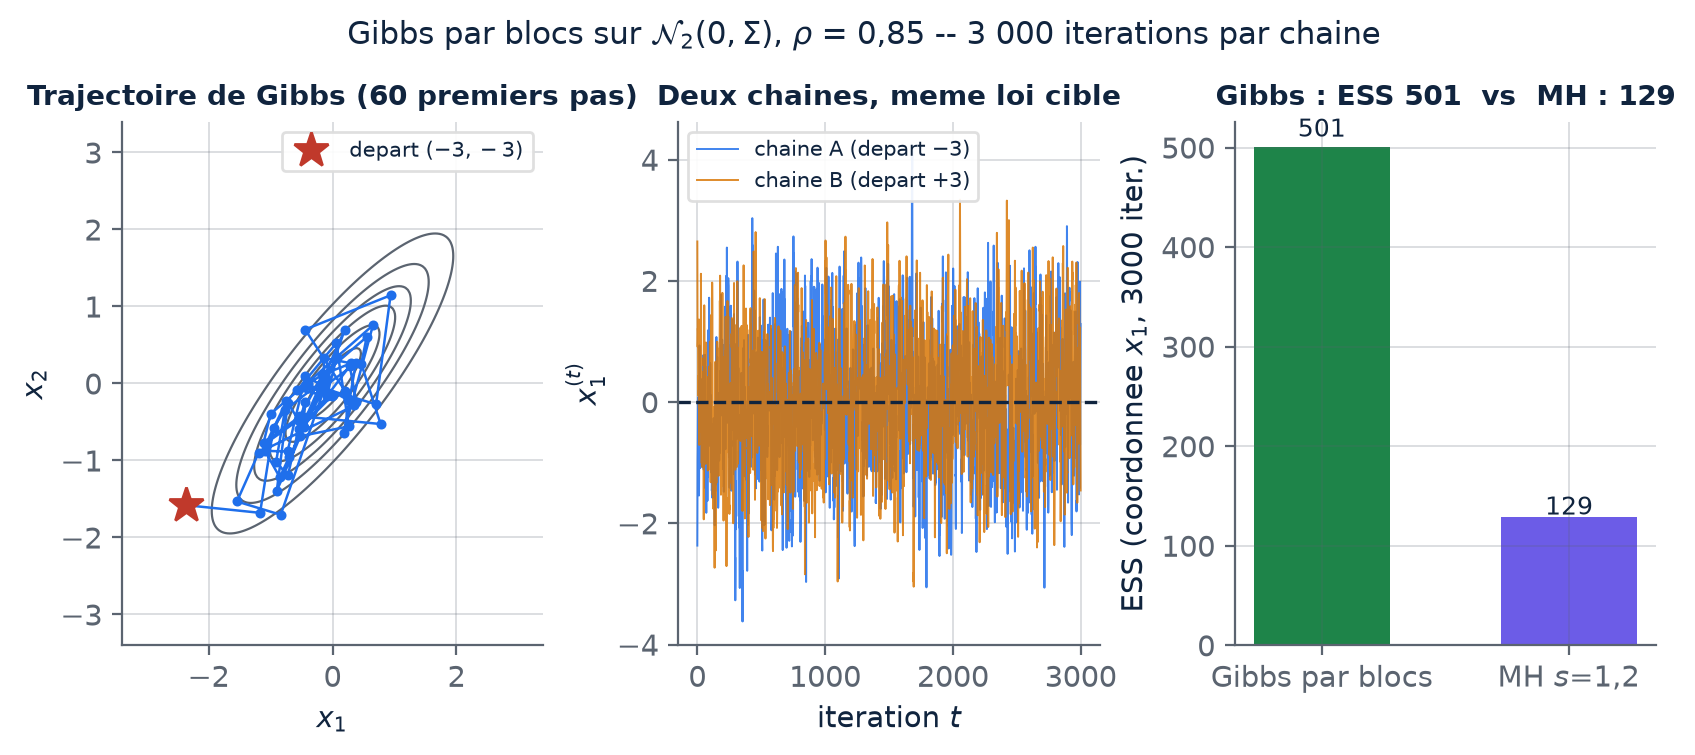
\includegraphics[width=.86\textwidth]{j07_gibbs_bivarie.png}
\end{center}
\end{frame}

% [split]
\begin{frame}{Gibbs exécuté : trajectoire et oubli de l'état initial}

\vspace{-2.5mm}
\begin{columns}[t]
\begin{column}{0.53\textwidth}
\begin{solbox}[Chiffres réels (script \file{src/fig\_ch5.py})]
\begin{itemize}
  \item Cible : $\N_2$ de corrélation 0,85 ; 3 000 itérations par chaîne.
  \item Trajectoire : de \emph{marches en escalier} (alternance
        verticale/horizontale) --- signature visuelle de Gibbs.
  \item Deux chaînes parties de $(-3,-3)$ et $(+3,+3)$ : la trace de $x_1$
        oublie le départ en quelques dizaines d'itérations.
  \item Moyenne obtenue : $-0{,}0272$ (vraie valeur 0) ; écart-type 1,0052
        (vraie valeur 1) ; corrélation 0,8465 (vraie valeur 0,85).
\end{itemize}
\end{solbox}
\end{column}
\begin{column}{0.45\textwidth}
\begin{qbox}[Question à se poser devant la figure]
Pourquoi la trajectoire de gauche ne se déplace-t-elle \textbf{jamais} en
diagonale ?
\vspace{1mm}
\\ \footnotesize Parce que le bloc mis à jour \emph{conditionne} sur la valeur
courante de l'autre bloc : on bouge un axe à la fois. Quand $\rho \to 1$, la cible
est un cigare très fin et Gibbs \emph{rame} le long du cigare.
\end{qbox}
\end{column}
\end{columns}
\end{frame}

% ---------------------------------------------------------------- 23
\begin{frame}{Gibbs : forces et faiblesses structurelles}
\footnotesize
\begin{columns}[t]
\begin{column}{0.49\textwidth}
\begin{kbox}[Forces]
\begin{itemize}
  \item \textbf{Aucun réglage} : pas de $s$, pas de $\varepsilon$, donc pas de
        phase d'adaptation.
  \item Tirages \textbf{exacts} à chaque bloc : acceptation 100 \%, et le
        posterior de chaque bloc est correctement échantillonné.
  \item Idéal pour les modèles à \textbf{structure conditionnelle simple} :
        régressions hiérarchiques, modèles à effets aléatoires, mélanges,
        modèles graphiques.
  \item Fournit naturellement un échantillonnage \emph{par blocs} : on ne
        simule que des lois de petite dimension.
\end{itemize}
\end{kbox}
\end{column}
\begin{column}{0.49\textwidth}
\begin{wbox}[Faiblesses]
\begin{itemize}
  \item Il faut connaître les \textbf{conditionnelles complètes} :
        \py{pm.Gibbs} n'existe pas pour un modèle écrit en langage PyMC --- on
        implémente Gibbs soi-même (conjugaison) ou on passe à NUTS.
  \item \textbf{Corrélations fortes} : le mouvement en escalier explore mal les
        directions obliques. Estimations numériques de référence : pour
        $\rho = 0{,}5$ l'ESS relatif reste élevé, mais pour $\rho \to 0{,}99$ il
        s'effondre ; c'est le reproche classique fait à Gibbs.
  \item \textbf{Multimodalité} : la chaîne reste dans un mode, et aucun
        réglage ne l'en fait sortir.
  \item Quand des composantes sont \textbf{très dépendantes} (centrée/non centrée),
        le choix de paramétrisation change tout (slide 30).
\end{itemize}
\end{wbox}
\end{column}
\end{columns}
\end{frame}

% ---------------------------------------------------------------- 24
\begin{frame}{De MH à HMC : et si la géométrie nous aidait ?}
% [rogna]
\footnotesize
\begin{columns}[t]
\begin{column}{0.5\textwidth}
\begin{ebox}[Le problème que MH et Gibbs ne résolvent pas]
\begin{itemize}
  \item Une marche aléatoire \textbf{découvre} la cible par tâtonnement
        ($\varepsilon$ : pas, direction tirée au hasard).
  \item Dans une direction étroite il faut de petits pas
        ($\varepsilon$), dans une direction large on avance trop lentement.
  \item Pour un modèle à 50 paramètres, la fraction de propositions acceptées
        s'effondre : c'est la \emph{malédiction de la dimension} des marcheurs
        aléatoires.
\end{itemize}
\end{ebox}
\end{column}
\begin{column}{0.48\textwidth}
\begin{kbox}[L'idée hamiltonienne]
Le \textbf{gradient} de $\log \tilde\pi$ indique où la densité augmente : au lieu
de proposer au hasard, on \emph{propose dans la bonne direction}, et suffisamment
loin.
\\[1mm]
On introduit un moment artificiel $p$ et l'on intègre une trajectoire physique
conservant l'\textbf{énergie}
\[
H(q,p) = \underbrace{-\log \tilde\pi(q)}_{U(q)}
\;+\; \underbrace{\tfrac12 p^{\!\top}p}_{K(p)}
\]
\centering\footnotesize $U$ : énergie potentielle ; $K$ : énergie cinétique.
Un mouvement conservatif visite la cible \emph{sans} errer : les propositions
lointaines deviennent très souvent acceptées.
\end{kbox}
\end{column}
\end{columns}
\vspace{1mm}
\begin{tcolorbox}[colback=byCyan!8,colframe=byCyan,arc=2mm,width=.96\textwidth]
\small\centering
\textbf{Coût du progrès :} HMC demande le gradient. En pratique, et c'est le cas
dans PyMC, ce gradient est obtenu par \textbf{différenciation automatique} du
log-posterior --- aucune dérivée n'est écrite à la main.
\end{tcolorbox}
\end{frame}

% ---------------------------------------------------------------- 25
\begin{frame}{Dynamique hamiltonienne expliquée (et vérifiée à l'écran)}
\footnotesize
\begin{columns}[t]
\begin{column}{0.52\textwidth}
\begin{ebox}[Les deux équations]
\[
\frac{\mathrm{d}q}{\mathrm{d}t} = \frac{\partial H}{\partial p} = p,
\qquad
\frac{\mathrm{d}p}{\mathrm{d}t} = -\frac{\partial H}{\partial q}
= \nabla \log \tilde\pi(q).
\]
L'état parcourt une courbe de \textbf{niveau d'énergie constant} : il glisse dans
les vallées du log-posterior. Deux propriétés sont préservées exactement par la
dynamique continue : le volume (théorème de Liouville) et l'énergie.
\end{ebox}
\begin{kbox}[La distribution cible en sort gratuitement]
Si $p \sim \N(0, I)$ et si l'on part de $q$ quelconque, alors $q$ \emph{après} la
trajectoire est distribué selon $\pi$ : le moment joue le rôle d'une variable
auxiliaire jetable. C'est une \textbf{augmentation} de la cible, exactement comme
au chapitre 2 pour les variables latentes.
\end{kbox}
\end{column}
\begin{column}{0.46\textwidth}
\begin{center}
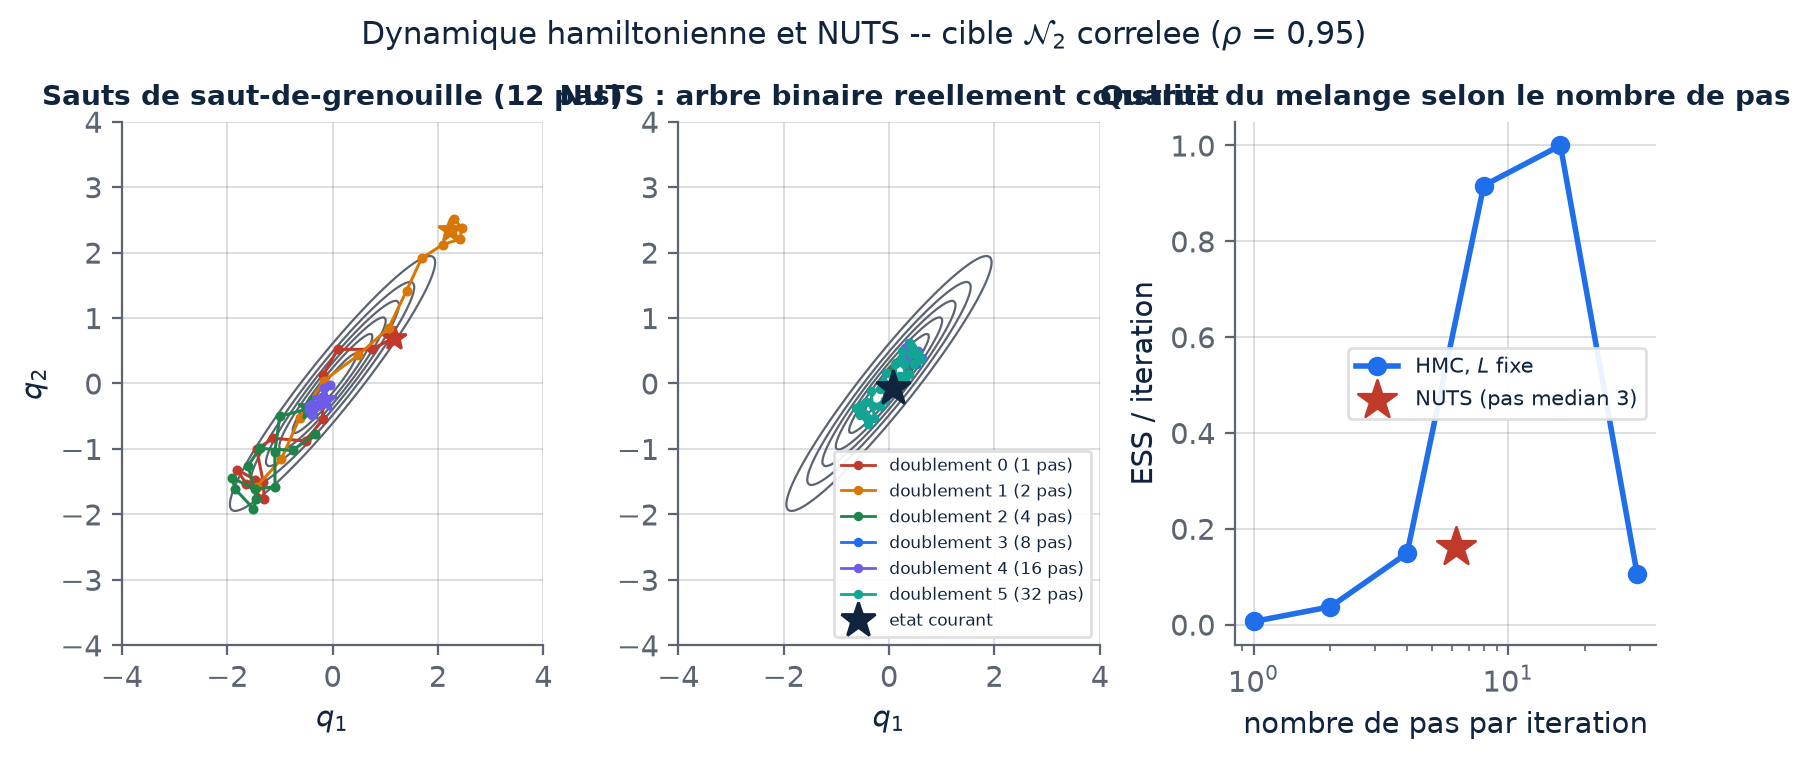
\includegraphics[width=\textwidth]{j08_hmc_nuts.png}
\end{center}
\vspace{-2mm}
\centering\footnotesize
Sauts de saut-de-grenouille (12 pas, $\varepsilon = 0{,}30$) sur une cible
$\N_2$ de corrélation 0,95 ; à droite, le doublement d'arbre de NUTS.
\end{column}
\end{columns}
\end{frame}

% ---------------------------------------------------------------- 26
\begin{frame}[fragile]{Saut-de-grenouille : l'intégrateur en dix lignes}
\footnotesize
\begin{columns}[t]
\begin{column}{0.53\textwidth}
\begin{codebox}[leapfrog.py --- intégrateur symplectique, exécuté]
\begin{lstlisting}
def leapfrog(q, p, eps, L, logp_grad):
    # p <- p + (eps/2) * grad log pi(q)
    qn, pn = q.copy(), p.copy()
    _, g = logp_grad(qn)
    pn += 0.5 * eps * g
    for _ in range(L - 1):        # L-1 pas complets
        qn += eps * pn
        _, g = logp_grad(qn)
        pn += eps * g
    qn += eps * pn                # dernier pas complet
    _, g = logp_grad(qn)
    pn += 0.5 * eps * g           # demi-pas final
    return qn, pn
\end{lstlisting}
\end{codebox}
\end{column}
\begin{column}{0.45\textwidth}
\begin{ebox}[Puis on corrige par Metropolis]
\begin{enumerate}
  \item tirer $p \sim \N(0, I)$ ;
  \item calculer $H_0 = -\log\tilde\pi(q) + \tfrac12 p^{\!\top}p$ ;
  \item intégrer $L$ pas : $(q,p) \to (q^\star, p^\star)$ ;
  \item calculer $H_1$ au nouveau point ;
  \item accepter avec probabilité $\min\!\big(1, e^{H_0 - H_1}\big)$.
\end{enumerate}
\end{ebox}
\begin{kbox}[Ce qu'il faut retenir du code]
\small
Le \emph{demi-pas} au début et à la fin n'est pas une coquetterie : c'est ce qui
rend l'intégrateur \textbf{symplectique} et \textbf{réversible}, donc valide pour
la correction de Metropolis. Écrire les deux demi-pas entiers casse la
réversibilité et biaise l'échantillon.
\end{kbox}
\end{column}
\end{columns}
\end{frame}

% ---------------------------------------------------------------- 27
\begin{frame}{HMC exécuté : les chiffres, et le prix du pas $L$}
\footnotesize
\begin{columns}[t]
\begin{column}{0.49\textwidth}
\begin{solbox}[HMC maison, 3 000 itérations, $\varepsilon = 0{,}30$, $L = 10$]
\begin{tabular}{@{}ll@{}}
\toprule
quantité & mesure \\
\midrule
acceptation & \textbf{85,2 \%} \\
ESS sur $x_1$ & \textbf{3 000 / 3 000} \\
erreur d'énergie $|\Delta H|$ & $< 0{,}01$ \\
évaluations de gradient & 10 par tirage \\
ESS par évaluation & 0,100 \\
\bottomrule
\end{tabular}
\vspace{1.5mm}
\\ Le même tirage par MH réglé donne ESS = 128,8 sur 3 000 : HMC obtient ici
\textbf{23 fois plus} d'échantillons utiles, au prix du gradient.
\end{solbox}
\begin{kbox}[Le réglage de $L$, mesuré]
\begin{tabular}{@{}lrrrrrr@{}}
\toprule
$L$ & 1 & 2 & 4 & 8 & 16 & 32 \\
ESS & 13 & 75 & 298 & 1 833 & 2 000 & 213 \\
\bottomrule
\end{tabular}
\vspace{1mm}
\\ Trop court, la trajectoire n'avance pas (ESS 13) ; trop long, elle revient sur
ses pas (ESS retombe à 213). Il faut donc régler $L$ --- sauf avec NUTS.
\end{kbox}
\end{column}
\begin{column}{0.49\textwidth}
\begin{qbox}[Pourquoi ne pas toujours prendre $L$ énorme ?]
\begin{itemize}
  \item Chaque pas coûte une évaluation du gradient : le budget est
        proportionnel à $L$.
  \item Au-delà d'un demi-tour de la cible, la trajectoire \textbf{rebrousse
        chemin} : on paie des pas qui ramènent près du départ.
  \item Mesure : $L = 16$ donne ESS = 2 000 pour 32 000 évaluations ; $L = 8$
        donne ESS = 1 833 pour 16 000 évaluations --- \emph{deux fois} moins
        cher pour un résultat quasi identique.
\end{itemize}
\end{qbox}
\end{column}
\end{columns}
\end{frame}

% ---------------------------------------------------------------- 28
\begin{frame}{NUTS : laisser la trajectoire décider}
\footnotesize
\begin{columns}[t]
\begin{column}{0.53\textwidth}
\begin{ebox}[No-U-Turn Sampler]
L'arbre est construit par \textbf{doublement} :
\begin{enumerate}
  \item partir de l'état courant, choisir au hasard un sens (avant/arrière) ;
  \item intégrer $2^0, 2^1, 2^2, \dots$ pas, garder un candidat tiré uniformément
        parmi les états retenus ;
  \item s'arrêter au \emph{U-turn} : $\langle q_+ - q_-, p_\pm \rangle < 0$.
\end{enumerate}
\end{ebox}
\begin{kbox}[Mesures sur la cible corrélée (corrélation 0,95), pas de 0,30]
\begin{tabular}{@{}ll@{}}
\toprule
pas par itération & médiane \textbf{3}, moyenne 6,2, maximum 15 \\
divergences & \textbf{0} sur 800 itérations \\
ESS sur $x_1$ & 129,9 sur 800, soit 0,162 par tirage \\
\bottomrule
\end{tabular}
\vspace{1mm}
\\ Sur cette cible 2D lisse, un $L$ bien réglé reste meilleur : NUTS paye le coût
d'explorer plusieurs longueurs. Son intérêt premier est de \textbf{supprimer le
réglage} et de rester efficace sur des cibles à courbure variable.
\end{kbox}
\end{column}
\begin{column}{0.48\textwidth}
\begin{qbox}[Et si l'on n'a pas le gradient ?]
Sur un modèle à \textbf{variables latentes discrètes} (allocation de mélange,
chaîne de Markov cachée), le gradient n'existe pas : on revient à Gibbs ou au
Metropolis à l'intérieur de Gibbs. NUTS n'est pas universel --- il exige un
log-posterior \textbf{différentiable}.
\end{qbox}
\end{column}
\end{columns}
\end{frame}

% ---------------------------------------------------------------- 29
\begin{frame}{Divergences : le diagnostic qui sauve une analyse}
\footnotesize
\begin{columns}[t]
\begin{column}{0.5\textwidth}
\begin{wbox}[Ce qu'est une divergence]
Sur une trajectoire, l'intégrateur doit conserver l'énergie : $|\Delta H|$
reste proche de 0. Une \textbf{divergence} est un pas où
$|\Delta H|$ explose (seuil usuel : $10^2$ à $10^3$) : la trajectoire est partie
dans une zone où la courbure est trop forte pour le pas $\varepsilon$.
\\[1mm]
Conséquence : le point est rejeté \emph{en silence} et l'on reste sur place.
La chaîne paraît acceptée correctement, mais elle \textbf{rate une région} du
posterior.
\end{wbox}
\begin{kbox}[Ce qu'il faut faire]
\begin{itemize}
  \item Elles sont \textbf{visibles} : \py{idata.sample_stats.diverging}.
  \item \textbf{Jamais} d'analyse sans avoir vérifié qu'il n'y en a pas.
  \item Remèdes, dans l'ordre : augmenter le \py{target\_accept}
        ($0{,}9 \to 0{,}99$), reparamétrer, simplifier le modèle.
\end{itemize}
\end{kbox}
\end{column}
\begin{column}{0.48\textwidth}
\begin{solbox}[Mesures du script --- funnel à 9 effets]
Toutes deux avec $\varepsilon = 0{,}25$, $L = 10$, 1 500 itérations :
\begin{tabular}{@{}lll@{}}
\toprule
& \textbf{centrée} & \textbf{non centrée} \\
\midrule
divergences & \textbf{17} (1,13 \%) & \textbf{0} \\
$|\Delta H|$ maximal & 812,5 & 0,10 \\
acceptation & 78,8 \% & 98,6 \% \\
ESS de $y$ & 33,8 & \textbf{286,7} \\
ESS / $N$ & 0,023 & \textbf{0,191} \\
\bottomrule
\end{tabular}
\vspace{1mm}
\\ Le même modèle, le même échantillonneur, le même budget : seule la
paramétrisation change, et l'efficacité est multipliée par 8.
\end{solbox}
\end{column}
\end{columns}
\end{frame}

% ---------------------------------------------------------------- 30
\begin{frame}{Reparamétrisation centrée contre non centrée : le funnel}
\footnotesize
\begin{center}
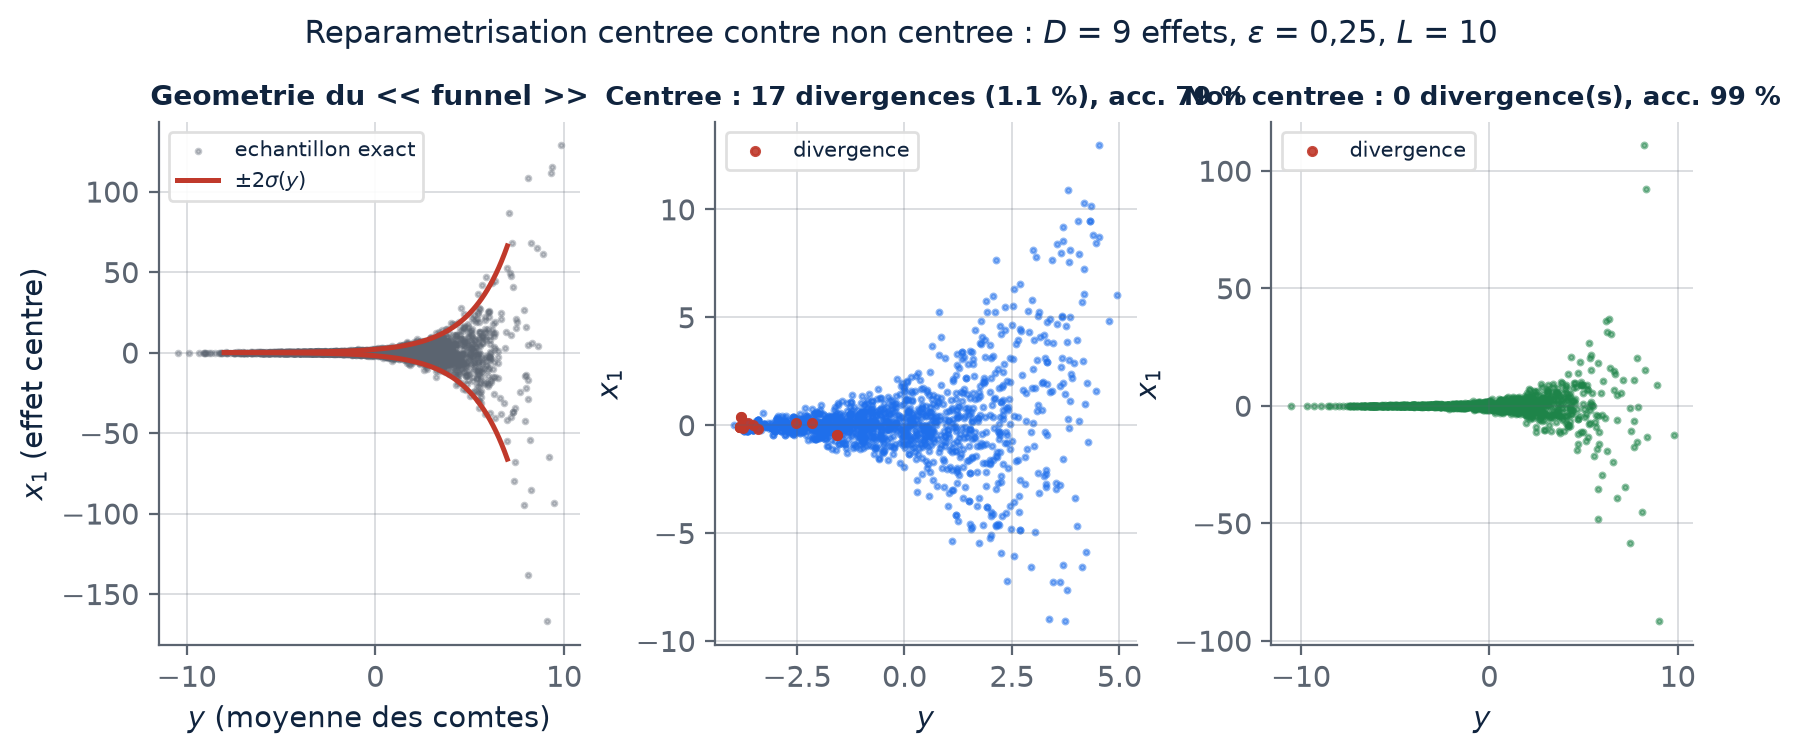
\includegraphics[width=.68\textwidth]{j09_funnel_centree.png}
\end{center}
\vspace{-3mm}
\begin{columns}[t]
\begin{column}{0.49\textwidth}
\begin{ebox}[Deux écritures du même modèle]
\textbf{Centrée :} $y \sim \N(0,3)$, \; $x_i \given y \sim \N\!\big(0, e^{y/2}\big)$ :
l'échelle des $x_i$ \emph{change avec} $y$, la densité dessine un entonnoir.
\\[1mm]
\textbf{Non centrée :} $y \sim \N(0,3)$, \; $z_i \sim \N(0,1)$,
\; $x_i = z_i\,e^{y/2}$ : la courbure vue par l'échantillonneur est constante.
\end{ebox}
\end{column}
\begin{column}{0.49\textwidth}
\begin{qbox}[Question de TP]
Dans un modèle hiérarchique $y_{ij} = a_j + b x_{ij} + \varepsilon$, quand
écrire $a_j \sim \N(\mu_a, \sigma_a)$ et quand
$a_j = \mu_a + \sigma_a z_j$, $z_j \sim \N(0,1)$ ?
\vspace{1mm}
\\ \footnotesize Règle : \textbf{peu} d'observations par groupe $\Rightarrow$
non centré ; \textbf{beaucoup} par groupe $\Rightarrow$ centré. Le mini-projet
tranche expérimentalement (section 5.5), et les mesures de la slide précédente
montrent l'enjeu : ESS multiplié par 8, divergences ramenées à 0.
\end{qbox}
\end{column}
\end{columns}
\end{frame}

% ---------------------------------------------------------------- 31
% [suite]
\begin{frame}{Choisir son échantillonneur : arbre de décision}
% [rogna]
\footnotesize
\begin{center}
\begin{tikzpicture}[every node/.style={font=\footnotesize},node distance=4mm,
  box/.style={draw,rounded corners,fill=byLight,inner sep=2.4mm,align=center},
  dec/.style={draw,diamond,aspect=2.2,fill=byOrange!12,inner sep=1mm,align=center}]
\node[dec] (q1) {les conditionnelles complètes\\sont-elles explicites ?};
\node[box,below left=9mm and 6mm of q1] (g) {\textbf{Gibbs} par blocs\\aucun réglage};
\node[dec,below right=9mm and 6mm of q1] (q2) {le gradient est-il\\disponible (autodiff) ?};
\node[box,below left=10mm and 2mm of q2] (mh) {\textbf{Metropolis-Hastings}\\+ adaptation de $s$};
\node[box,below right=10mm and 2mm of q2] (h) {\textbf{HMC / NUTS}\\+ $target\_accept$ élevé};
\node[box,below=16mm of q2,fill=byRed!10] (rep) {\textbf{Divergences ?} $\rightarrow$ reparamétriser (non centré),\\contrôler les échelles, simplifier};
\draw[-{Latex[length=2mm]}] (q1) -- node[above,font=\scriptsize]{oui} (g);
\draw[-{Latex[length=2mm]}] (q1) -- node[above,font=\scriptsize]{non} (q2);
\draw[-{Latex[length=2mm]}] (q2) -- node[above,font=\scriptsize]{non} (mh);
\draw[-{Latex[length=2mm]}] (q2) -- node[above,font=\scriptsize]{oui} (h);
\draw[-{Latex[length=2mm]}] (q2) -- (rep);
\end{tikzpicture}
\end{center}
\vspace{-3mm}
\end{frame}

% [suite]
\begin{frame}{Choisir son échantillonneur : arbre de décision (suite)}
\begin{columns}[t]
\begin{column}{0.49\textwidth}
\begin{abox}[Le réflexe industriel : NUTS par défaut]
Dans PyMC, \py{pm.sample()} appelle NUTS avec adaptation du pas. On ne choisit
donc pas son échantillonneur dans 90 \% des cas : on choisit sa
\textbf{paramétrisation} et son \py{target\_accept}. C'est là que passe
l'essentiel du temps de débogage.
\end{abox}
\end{column}
\begin{column}{0.49\textwidth}
\begin{wbox}[Trois signaux d'alerte]
\nok{} des \textbf{divergences}, même 2 ou 3 sur 4 000 tirages :\;
elles indiquent une zone non explorée.\\
\nok{} un $\hat R > 1{,}01$ sur un paramètre : \; ne tirez aucune conclusion.\\
\nok{} un ESS \textbf{inférieur à 100} pour un paramètre d'intérêt : \; l'intervalle
de crédibilité sera instable d'une exécution à l'autre.
\end{wbox}
\end{column}
\end{columns}
\end{frame}

% ---------------------------------------------------------------- 32
\begin{frame}{Exercice encadré : régler une proposition comme un pro}
\footnotesize
\begin{abox}[Consigne (15 min, binôme, machine)]
Reprendre le MH maison de la slide 15 sur la cible Beta$(2{,}5\,;\,7)$ et :
\begin{enumerate}
  \item écrire une boucle qui teste $s \in \{0{,}01 ; 0{,}02 ; 0{,}05 ; 0{,}1 ;
        0{,}2 ; 0{,}35 ; 0{,}6 ; 1{,}0 ; 1{,}8 ; 3{,}0 ; 6{,}0\}$ sur 20 000 itérations ;
  \item tracer l'ESS en fonction de $s$ et marquer le maximum ;
  \item vérifier que l'ESS maximal est atteint pour $s \approx 0{,}35$ et que
        l'acceptation y vaut environ 41 \% ;
  \item refaire l'expérience avec une proposition \emph{uniforme}
        $\theta^\star \sim \mathrm{U}(\theta - s, \theta + s)$ et comparer les ESS ;
  \item conclure : quelle famille de propositions choisir et pourquoi.
\end{enumerate}
\end{abox}
\vspace{1mm}
\begin{columns}[t]
\begin{column}{0.49\textwidth}
\begin{solbox}[Résultats de référence (attendus)]
$s$ optimal mesuré : \textbf{0,35}, ESS = \textbf{4 070} sur 20 000
(soit 0,204 par tirage), acceptation 41,4 \%. Le pire cas mesuré est
$s = 0{,}01$ : ESS = \textbf{21}, acceptation 97,6 \%.
\end{solbox}
\end{column}
\begin{column}{0.49\textwidth}
\begin{kbox}[Ce que l'exercice fait comprendre]
Un pas trop grand \emph{et} un pas trop petit sont deux échecs symétriques. Le
critère de jugement n'est jamais le taux d'acceptation seul : c'est l'ESS
(lui-m\^eme estimé sur une chaîne assez longue pour être fiable).
\end{kbox}
\end{column}
\end{columns}
\end{frame}

% ---------------------------------------------------------------- 33
\begin{frame}{Synthèse 5.3 --- Gibbs, HMC et NUTS}
\footnotesize
\begin{columns}[t]
\begin{column}{0.52\textwidth}
\begin{tcolorbox}[enhanced,colback=byPurple!7,colframe=byPurple,arc=2mm,
   title={\bfseries\color{white}\faLightbulb\ Synthèse},colbacktitle=byPurple,
   attach boxed title to top left={xshift=3mm,yshift=-2mm},
   boxed title style={arc=1mm,boxrule=0pt}]
\begin{itemize}
  \item \textbf{Gibbs} : exact, sans réglage, imbattable si les conditionnelles
        sont closes --- ESS 0,167 par tirage contre 0,043 pour MH sur la même cible.
  \item \textbf{HMC} : le gradient transforme la marche aléatoire en trajectoire
        physique (acceptation 85 \%, ESS = 3 000 sur 3 000 tirages, mais
        10 évaluations de gradient par tirage).
  \item Le réglage de $L$ est un vrai piège (ESS : 13 pour $L = 1$, 2 000 pour
        $L = 16$, 213 pour $L = 32$) ; \textbf{NUTS} le supprime par doublement
        d'arbre (médiane 3 pas ici).
  \item \textbf{Divergences} et \textbf{reparamétrisation} : sur le funnel,
        17 divergences et ESS/\,$N$ = 0,023 en centré contre \textbf{0 divergence
        et ESS/\,$N$ = 0,191} en non centré --- à modèle identique.
\end{itemize}
\end{tcolorbox}
\end{column}
\begin{column}{0.46\textwidth}
\begin{abox}[À faire avant la séance 6]
\begin{itemize}
  \item Reproduire les trois échantillonneurs maison
        (\file{src/fig\_ch5*.py}) et vérifier les ordres de grandeur du tableau.
  \item Refaire le funnel avec $D = 1$ (un seul effet) : les divergences
        disparaissent-elles ? Pourquoi ?
  \item Sur une cible $\N_2$ de corrélation 0,99, comparer Gibbs et HMC :
        qui gagne, et de combien ?
  \item Lire \py{az.plot_rank} sur les chaînes HMC produites.
\end{itemize}
\end{abox}
\begin{tcolorbox}[colback=byCyan!8,colframe=byCyan,arc=2mm]
\small\textbf{Fil rouge :} tout échantillonneur est jugé sur \emph{trois}
choses --- la justesse (invariance), l'efficacité (ESS), la couverture
(aucune zone perdue : divergences, chaînes multiples).
\end{tcolorbox}
\end{column}
\end{columns}
\end{frame}
